\section{一定ベット}
まずは、賭け金を常に一定として、所持金がどのように変化するのかをシミュレーションで調べる。シミュレーション結果を図\ref{betdife}と表\ref{bet}で示す。
\begin{figure}[H]
 \begin{center} 
  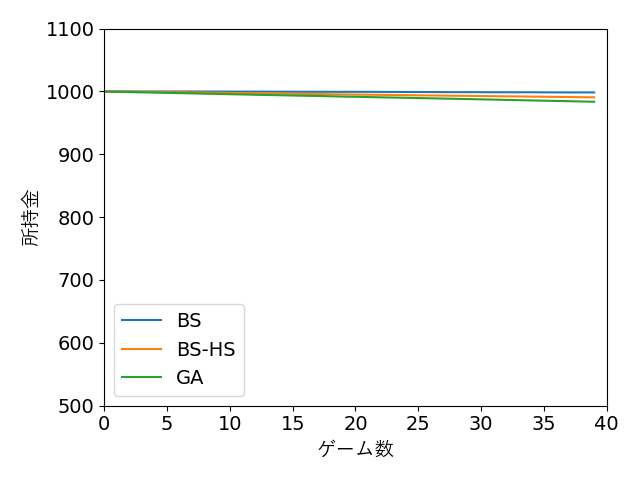
\includegraphics[width=0.7\linewidth]{./figure/bet-defineite-ver5}
  \caption{一定ベット\label{betdife}}
 \end{center}
\end{figure}

\begin{table}[H]
 \caption{一定ベットの所持金\label{bet}}
 \begin{center}
  \begin{tabular}{|c|c|c|}
  \hline  & 40回目の平均所持金 & 標準偏差 \\
  \hline BS & 998.328 & 73.538\\
  \hline BS-HS & 990.499 & 62.013 \\
  \hline GA戦略 & 983.470 & 62.401\\
  \hline
  \end{tabular}
 \end{center}
\end{table}

このシミュレーションでは最初の所持金を1000とし、常に10賭け、ブラックジャックの勝負を連続で40回行い、それを5万回行った。また戦略はダブルダウンやスプリットなどが入ったベーシックストラテジー(BS)とヒットとスタンドのみのベーシックストラテジー(BS-HS)、GAで作成した戦略(GA戦略)の3つを使用した。
 図\ref{betdife}では所持金は勝負を重ねるたびに少しずつ少なくなっていて、最後の40回目では最初の所持金である1000より少し少なくなっているように見える。そこで表\ref{bet}を見ると40回目のそれぞれの所持金が分かるが、ダブルダウンやスプリットが入ったベーシックストラテジー、ヒットとスタンドのみのベーシックストラテジー、GA戦略の順で多いことが分かる。どの戦略でも最初の所持金である1000を超えることはないことが分かった。\\
 賭け金が一定では最初の所持金を超えることができなかった。そのため賭け金を変動させることが必要だと考えた。まず、この勝負40回の中で勝率が変動するところがないかを確認した。勝負のどこかで勝率が高くなれば賭け金をあげ、低くなれば賭け金を下げることで所持金を増やそうと考えたためである。また、カウンティングという手法を用いてみるという2つの手法を考えた。
\bunseki{※柿崎大輝}

\subsection{勝率の推移}
ブラックジャックを連続で行った場合で勝率は変化を調べる。シミュレーション結果を図\ref{win}で示す。
\begin{figure}[H]
 \begin{center} 
  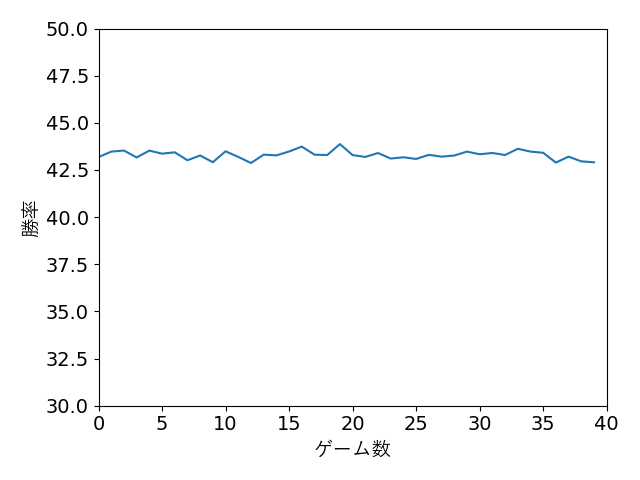
\includegraphics[width=0.7\linewidth]{./figure/win}
  \caption{勝率の推移\label{win}}
 \end{center}
\end{figure}
ブラックジャックの勝負を連続で40回行い、それを5万回繰り返して、勝負ごとでの勝率を調べた。デック数は6で、使用した戦略はヒットとスタンドのみのベーシックストラテジーであった。
図\ref{win}を見ると勝率は42\%~44\%の間で増減を繰り返しており、だいたい43\%の部分に集中していると分かる。勝率は特に目立った規則性は見られず、ランダムに増減を繰り返しているように見られる。勝率は最高で43.87\%で最低は42.868\%であった。
 シミュレーション結果から勝率は勝負40回の中であまり変化しないと考えられる。また、勝率の変動に規則性は見つからなかった。そのため、勝負のどこかで賭け金を増やすという戦略はできないということが分かった。
\bunseki{※柿崎大輝}

\subsubsection{カイ2乗検定}
40回の勝負で1つ1つを比べてみて、勝率の差は小さいものであった。しかし、本当にその差には意味がないのか、小さくても本当は意味がある差なのではないか。それを確かめるために、カイ2乗検定を行い、勝率の差が有意な差であるかどうかを確かめる。
 カイ2乗検定を行う前に必要な条件を表\ref{win-x}でまとめる。
\begin{table}[H]
 \caption{勝率の差のカイ2乗検定条件\label{win-x}}
 \begin{center}
  \begin{tabular}{|c|c|}
  \hline 帰無仮説 & 勝率の差に有意な差がない \\
  \hline 対立仮説 & 勝率の差に有意な差がある \\
  \hline 有意水準 & 5\% \\
  \hline 自由度 & 39 \\
  \hline 棄却値 & 54.57\\
  \hline
  \end{tabular}
 \end{center}
\end{table}
有意水準5\%で、棄却値は54.57とした。カイ2乗値がこの棄却値54.57より大きければ帰無仮説を棄却し、対立仮説を採択する。
 ここで、カイ2乗検定を行うとカイ2乗値は40.207となった。カイ2乗値は棄却値よりも小さくなったので、帰無仮説を採択する。よって、勝率の差には有意な差がないという結果になった。つまり、勝負40回で勝率の変化はないという結果となった。
\bunseki{※柿崎大輝}

\section{カウンティング}
カウンティングで賭け金を変動させ、所持金を調べる。カウンティングは既存のカウンティング手法としてKO法とHigh-Low法の2種類とプロジェクトで作成したカウンティング手法のRUKO法と5-6-A法の2種類、計4種類を用いる。そのほかの条件は一定ベットの時のシミュレーションと同じとした。シミュレーション結果を図\ref{KO}と図\ref{Hi-Lo}と表\ref{countting}で示す。
\begin{figure}[H]
 \begin{center} 
  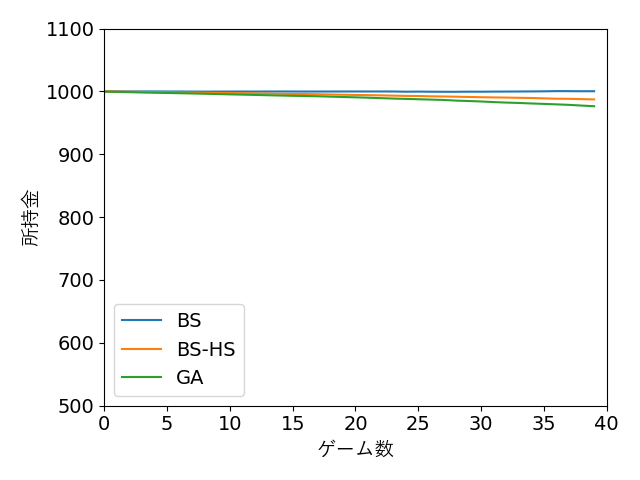
\includegraphics[width=0.7\linewidth]{./figure/KO}
  \caption{カウンティングKO法\label{KO}}
 \end{center}
\end{figure}

\begin{figure}[H]
 \begin{center} 
  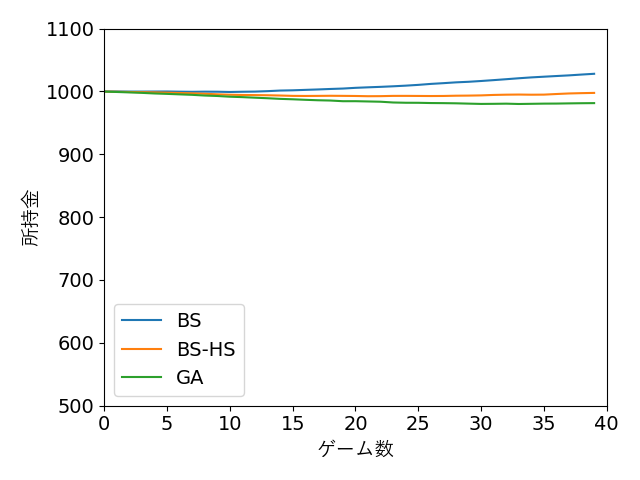
\includegraphics[width=0.7\linewidth]{./figure/Hi-Lo}
  \caption{カウンティングHigh-Low法\label{Hi-Lo}}
 \end{center}
\end{figure}

\begin{figure}[H]
 \begin{center} 
  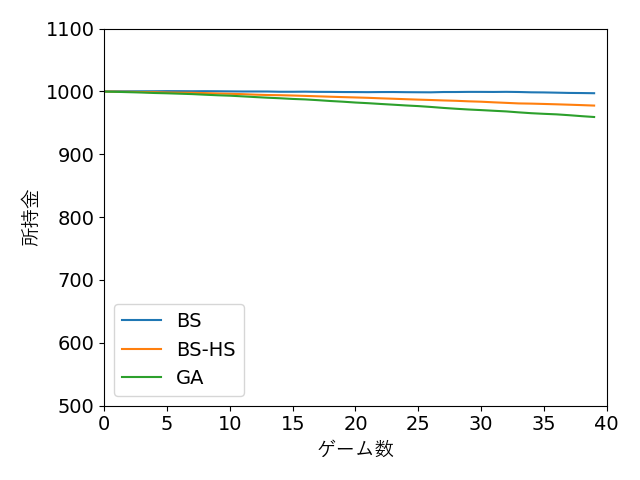
\includegraphics[width=0.7\linewidth]{./figure/RUKO}
  \caption{カウンティングRUKO法\label{RUKO}}
 \end{center}
\end{figure}

\begin{figure}[H]
 \begin{center} 
  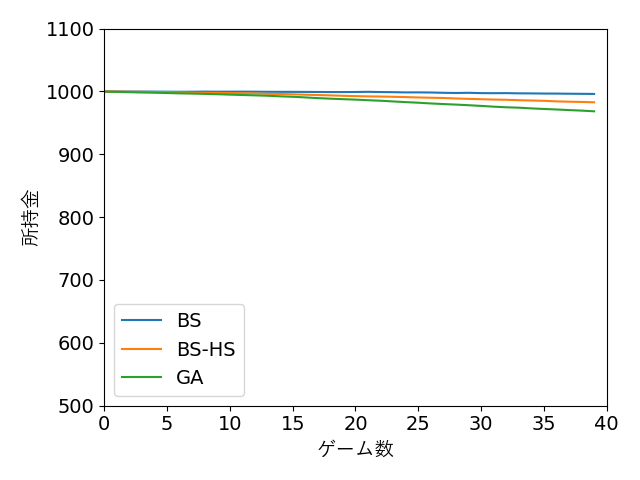
\includegraphics[width=0.7\linewidth]{./figure/56A}
  \caption{カウンティング5-6-A法\label{56A}}
 \end{center}
\end{figure}

\begin{table}[H]
 \caption{カウンティングの所持金\label{countting}}
 \begin{center}
  \begin{tabular}{|c|c|c|}
  \hline  & 40回目の平均所持金 & 標準偏差 \\
  \hline KO法BS & 1000.237 & 172.770\\
  \hline KO法BS-HS & 987.207 & 148.615 \\
  \hline KO法GA戦略 & 976.380 & 145.821\\
  \hline High-Low法BS & 1027.961 & 298.197\\
  \hline High-Low法BS-HS  & 997.561 & 262.546\\
  \hline High-Low法GA戦略 & 981.315 & 263.162\\
  \hline RUKO法BS & 1000.237 & 172.770\\
  \hline RUKO法BS-HS & 987.207 & 148.615 \\
  \hline RUKO法GA戦略 & 976.380 & 145.821\\
  \hline 5-6-A法BS & 995.918 & 211.884\\
  \hline 5-6-A法BS-HS & 982.640 & 179.584 \\
  \hline 5-6-A法GA戦略 & 968.303 & 180.464\\
  \hline
  \end{tabular}
 \end{center}
\end{table}

KO法は図\ref{KO}で見ると一定ベットの時とあまり変化がないように見えるが、表\ref{countting}で見るとダブルダウンやスプリットが入ったベーシックストラテジーの所持金が増加していることが分かる。
 High-Low法は図\ref{Hi-Lo}ではで増えていることがはっきりと分かる。表\ref{countting}で見てもすべての戦略で一定ベットの時よりも増えていることが分かる。しかし、標準偏差が一定ベットやKO法の2つより大きく、安定していないことが分かる。
 既存のカウンティング手法を使うことでダブルダウンやスプリットが入ったベーシックストラテジーでは1000を超えることができた。ただ、ヒットとスタンドのみのベーシックストラテジーやGA戦略では1000を超すことはできなかった。\\
 RUKO法:ここにRUKOの結果\\
 5-6-A法:ここに5-6-Aの結果\\
 上2つのまとめ\\
 カウンティング手法全部のまとめ\\
 ここで注目するのはGA戦略である。一定ベットやカウンティングを使用しても所持金がすべての戦略で一番少なかった。GA戦略は遺伝子アルゴリズムで探索し、発見した戦略であるのになぜ他の戦略より悪い結果となったのか。それは複雑性ということを考慮していないからではないかと考えた。GA戦略は勝率と複雑性からなる性能で探索したもので、行ったシミュレーションでは複雑性を考慮する部分がなく、その結果一番悪い結果となったと考えた。そこで複雑性を確かめる実験の結果を用いて、"エラー率"という指標を作成し、シミュレーションに導入して行うこととした。
\bunseki{※柿崎大輝}

\section{エラー率の導入}
GA戦略が結果として最も低い所持金となった原因は、シミュレーションを行う条件にあった。GA戦略は複雑性が低い、つまりシンプルであることが最大の特徴である。そこで、我々はGA戦略の特徴がどのくらい有用かを調べるために複雑性を考慮したシミュレーションを行う必要があった。そして、そのシミュレーションを行うため、複雑性に関する実験の結果をもとにエラー率という概念を作成した。エラー率の定義は、ある戦略を使用する際にプレイヤーが行動を間違えてしまう確率を表したものである。このエラー率をシミュレーションに適用することにより、GA戦略を使用した際のプレイヤーの所持金が良い方向に改善される可能性があるのではないかと考えた。このエラー率の導出方法として、複雑性に関する実験データの正答率をもとに線形回帰分析を行った。また、使用した実験データについては以下の\ref{hoge}で示す通りである。

  \begin{table}[H]
    \begin{tabular}{lllll}
      複雑性&0.2&0.2&0.407&0.448 \\
      エラー率&0.002&0.009&0.125&0.162 \\ 
    \end{tabular}
    \caption{複雑性と誤答率}
    \label{hoge}
  \end{table}
また、以上の実験データから線形回帰分析により得られた式は、

  \begin{equation}
    y=0.611x - 0.1172
  \end{equation}

となった。この式を横軸を複雑性、縦軸をエラー率としてグラフにしたものが図\ref{hoge2}である。

  \begin{figure}[H]
    \label{hoge2}
    \begin{center}
      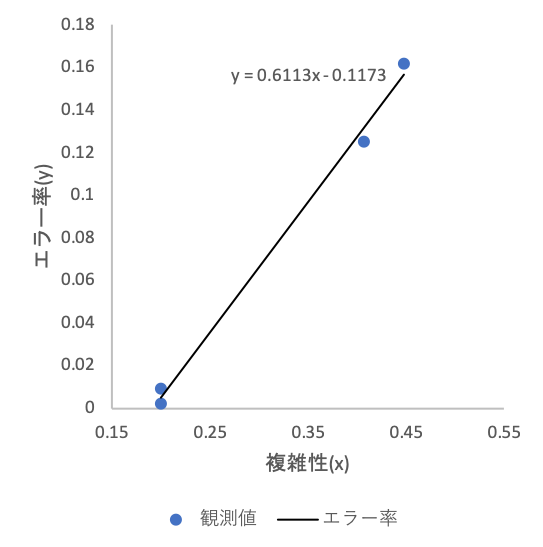
\includegraphics[width=10cm]{figure/error_rate.png}
      \caption{線形回帰分析によるエラー率のグラフ}
    \end{center}
  \end{figure}
\bunseki{※薩田凱斗}

\section{エラー率を導入したシミュレーション}
エラー率を導入して、シミュレーションを行う。エラー率は戦略に従って行動するときにミスをする確率で、ミスをすると戦略表とは異なる行動を実行するようにした。またカウンティング手法はKO法とHigh-Low法の2種類を用いた。それ以外の部分は前のシミュレーションと同じ条件とした。表\ref{err}が戦略ごとのエラー率で、図\ref{errKO}と図\ref{errHi-Lo}、表\ref{money-err}がシミュレーション結果である。
\begin{table}[H]
 \caption{戦略ごとのエラー率\label{err}}
 \begin{center}
  \begin{tabular}{|c|c|}
  \hline 戦略 & エラー率(\%) \\
  \hline BS & 16.2\\
  \hline BS-HS & 4.8 \\
  \hline GA戦略 & 0.5\\
  \hline
  \end{tabular}
 \end{center}
\end{table}

\begin{figure}[H]
 \begin{center} 
  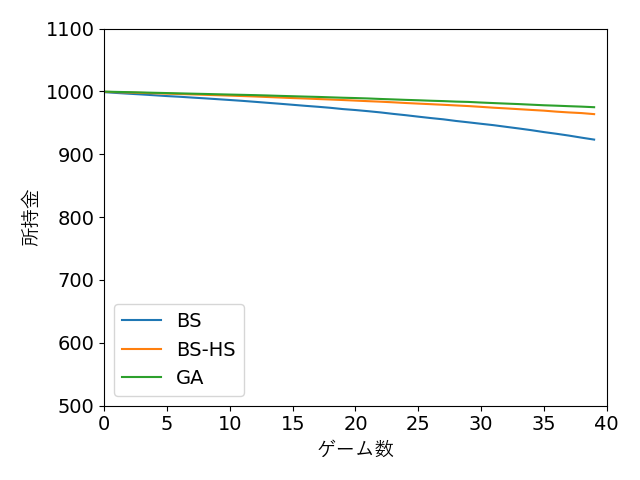
\includegraphics[width=0.7\linewidth]{./figure/errKO}
  \caption{エラー率ありのKO法\label{errKO}}
 \end{center}
\end{figure}

\begin{figure}[H]
 \begin{center} 
  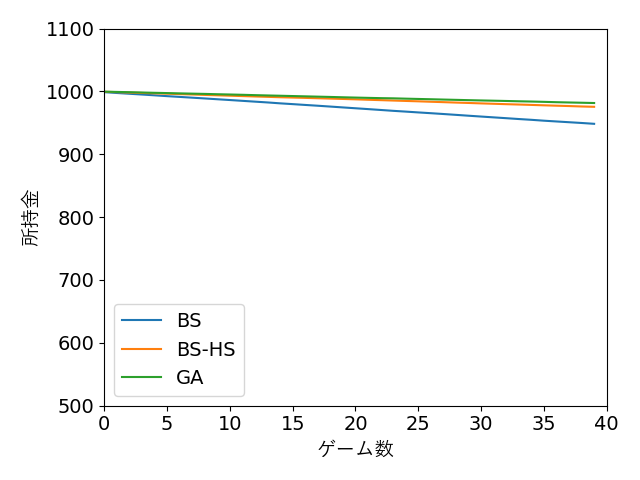
\includegraphics[width=0.7\linewidth]{./figure/errHi-Lo}
  \caption{エラー率ありのHigh-Low法\label{errHi-Lo}}
 \end{center}
\end{figure}

\begin{table}[H]
 \caption{エラー率を使用した際の所持金\label{money-err}}
 \begin{center}
  \begin{tabular}{|c|c|c|}
  \hline  & 40回目の平均所持金 & 標準偏差 \\
  \hline KO法BS & 923.303 & 174.255\\
  \hline KO法BS-HS & 963.799 & 150.135 \\
  \hline KO法GA戦略 & 974.817 & 144.821\\
  \hline High-Low法BS & 948.394 & 79.764\\
  \hline High-Low法BS-HS  & 975.440 & 67.263\\
  \hline High-Low法GA戦略 & 981.474 & 67.747\\
  \hline
  \end{tabular}
 \end{center}
\end{table}
エラー率を導入した結果ではGA戦略、ヒットとスタンドのみのベーシックストラテジー、ダブルダウンやスプリットが入ったベーシックストラテジーの順となり、所持金が1番多かったダブルダウンやスプリットが入ったベーシックストラテジーと1番少なかったGA戦略が入れ替わった。特にダブルダウンやスプリットが入ったベーシックストラテジーはエラー率を導入することで大きく所持金が少なくなった。またエラー率を導入したシミュレーションでは1000を超える戦略はないことが分かった\\
 エラー率を導入した場合、GA戦略が1番優れていることが分かった。しかし、GA戦略では1000を超えることができないことも分かった。この点にGA戦略は改善がする必要があると考えられる。
\bunseki{※柿崎大輝}

\subsection{分散分析}
エラー率を導入したシミュレーションの時、3つの戦略間で40回目の平均所持金に有意な差があるかどうかを調べる。まず、3つの戦略において有意な差があるかどうかを調べるため、分散分析を行った。優位水準は5\%、KO法とHigh-Low法の2種類で行った。表\ref{conditions-b}で分散分析の条件をまとめた。
\begin{table}[H]
 \caption{分散分析の条件\label{conditions-b}}
 \begin{center}
  \begin{tabular}{|c|c|}
  \hline 帰無仮説 & 3つの戦略で平均所持金に有意な差はない \\
  \hline 対立仮説 & 3つの戦略で平均所持金に有意な差はある \\
  \hline 有意水準 & 5\% \\
  \hline
  \end{tabular}
 \end{center}
\end{table}
分散分析を行うと、KO法、High-Low法のp値がとても小さくなり、0.05以下となる。よって帰無仮説を棄却し、対立仮説を採択する。つまり、3つの戦略で有な差が存在することが確認できた。次は3つの戦略のどこに有意な差が存在するのかを調べるためにここから多重比較を行う。
\bunseki{※柿崎大輝}

\subsection{多重比較}
それぞれの戦略で有意な差があるかを調べため、多重比較を行った。有意水準を5\%として行った。結果は表\ref{multiKO}と表\ref{multiHigh-Low}に示す。
\begin{table}[H]
 \caption{KO法での多重比較\label{multiKO}}
 \begin{center}
  \begin{tabular}{|c|c|c|}
  \hline  & BS & BS-HS  \\
  \hline  BS-HS 所持金の差 & 40.496 & \\
	               p値 & 0 & \\
  \hline GA 所持金の差 & 51.515 & 11.019\\
                p値 & 0 & 0\\
  \hline
  \end{tabular}
 \end{center}
\end{table}
\begin{table}[H]
 \caption{KO法での多重比較\label{multiHigh-Low}}
 \begin{center}
  \begin{tabular}{|c|c|c|}
  \hline  & BS & BS-HS  \\
  \hline  BS-HS 所持金の差 & 27.046 & \\
	               p値 & 0 & \\
  \hline GA 所持金の差 & 33.080 & 6.034\\
                p値 & 0 & 0\\
  \hline
  \end{tabular}
 \end{center}
\end{table}
 表\ref{multiKO}と表\ref{multiHigh-Low}ではそれぞれの戦略を比較した場合の所持金の差とp値を表示している。所持金がプラスの場合は列側の戦略のほうが所持金が多く、逆にマイナスなら行側の戦略のほうが所持金が多い。また、p値が0.05より小さい場合、その2つの戦略で有意な差が存在するということが分かる。\\
 KO法ではすべての戦略間でp値が0.05以下となり、すべての戦略間で有意な差が存在することが分かった。High-Low法でもすべての戦略間でp値が0.05以下となり、すべての戦略間で有意な差が存在することが分かった。これでKO法High-Low法の両方ですべて戦略間で有意な差が存在する。
\bunseki{※柿崎大輝}